\chapter{Working with Binary-Valued Graph Signals} % Main chapter title

\label{chap:binary} 

\lhead{Chapter 7. \emph{Working with Binary-Valued Graph Signals}} 

So far in this thesis, we have focused on reconstruction and regression models for real-valued graph signals, as discussed in \cref{chap:gsr_2d,chap:kgr_rnc_2d,chap:nd_gsp,chap:variance}. In this chapter, we shift our attention to scenarios where the signal of interest is binary-valued. Such signals can be employed to describe node classification tasks conducted over networks. For instance, consider the task of predicting whether users in a social network will click on a specific online advertisement. It is reasonable to assume that closely connected individuals within the network are more likely to have a similar probability of clicking than distantly connected individuals. Consequently, integrating this relational information into a predictive task may enhance accuracy.

In this example, the classification task is binary as visualised in \cref{fig:binary_class_graph}. However, there may also be situations in which each node must be classified into more than two groups. In this case, we have a multiclass classification


\begin{figure}[t] 
    \begin{center}
        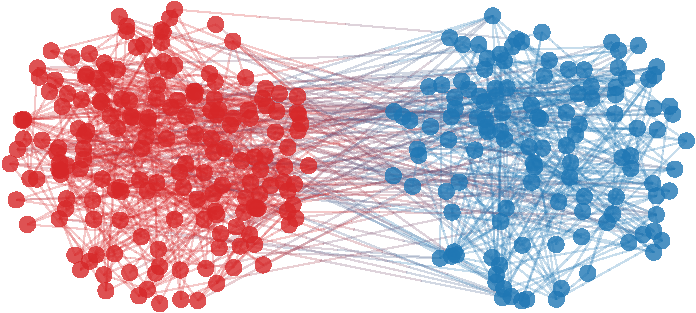
\includegraphics[width=0.8\linewidth]{Figures/2class_graph.pdf}
    \end{center}
   \caption[Visualisation of a binary classification task over a network]{An example visualisation of a binary classification task over a network.} 
    \label{fig:binary_class_graph}
\end{figure} 

\begin{figure}[t] 
    \begin{center}
        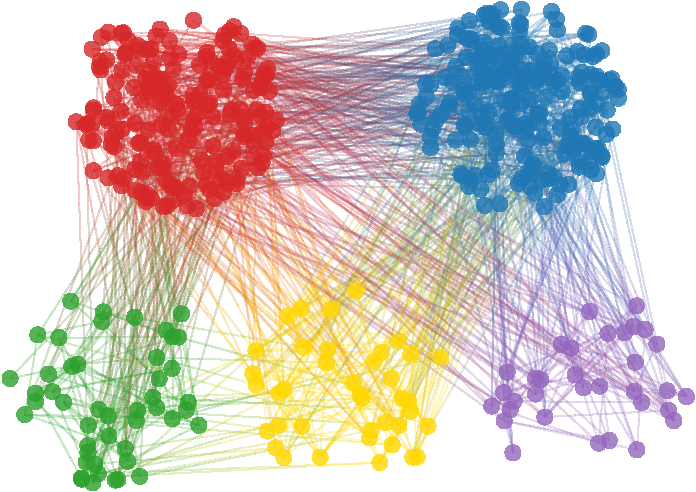
\includegraphics[width=0.8\linewidth]{Figures/multiclass_graph.pdf}
    \end{center}
   \caption[Visualisation of a multiclass classification task over a network]{An example visualisation of a multiclass classification task over a network.} 
    \label{fig:mutliclass_graph}
\end{figure} 



\section{Logistic Graph Signal Reconstruction}

\label{sec:lgsr}



Consider a binary signal reconstruction problem over a Cartesian product graph of order $d$. The observed graph signal, $\Yt$, is an order-$d$ tensor of shape $(N_1, N_2, .., N_d)$, with binary-valued elements. This is accompanied by another binary tensor, $\St$, of the same shape. As in previous chapters, $\St$ contains the information about which elements of $\Yt$ were observed by holding ones at elements where successful observations were made and zeros elsewhere. The goal is to predict the value of the graph signal at elements where no observation was made. 

\begin{equation*}
    \text{input data} = \Big\{\; \Yt \in \{0, 1\}^{N_1 \times ... \times N_d}, \;\; \St \in \{0, 1\}^{N_1 \times ... \times N_d} , \;\; \A \in \R^{N \times N} \; \Big\}
\end{equation*}

In the following, we assume each element, $\nn$, of the tensor, $\Yt$, follows a Bernoulli distribution, where the mean described by the value of $\Mt_\nn$. 

\begin{equation*}
    \Yt_\nn \sim \text{Bern}\left(\Mt_\nn \right)
\end{equation*}


$\Mt$ is another tensor, with the same shape as $\Yt$ and elements on the interval $[0, 1]$, and is characterised by the following expression. 

\begin{equation}
    \Mt \in [0, 1]^{N_1 \times ... \times N_d}= \frac{1}{1 + \exp(\Ft)}
\end{equation}

where $\Ft \in \R^{N_1 \times ... \times N_d}$ is a real-valued graph signal. As in previous chapters, we make the assumption that $\Ft$ is smooth with respect to the topology of the graph by assigning it the following prior. 

\begin{equation}
    \f = \vecrm{\Ft} \, \sim \, \mathcal{N}\left( \zero, \, \gamma^{-1} \HH^2 \right) 
\end{equation}



\cite{Li2012}

\section{Logistic Kernel Graph Regression}

 
\label{sec:lkgr}


\section{Logistic Regression with Network Cohesion}

\label{sec:lrnc}

\section{Multiclass Methods}

\label{sec:multiclass}


\section{Approximate Sampling via the Laplace Approximation}

\label{sec:lsamp}

